\documentclass[a4paper]{article}

%% Language and font encodings
\usepackage[english]{babel}
\usepackage[utf8x]{inputenc}
\usepackage[T1]{fontenc}

%% Sets page size and margins
\usepackage[a4paper,top=3cm,bottom=2cm,left=3cm,right=3cm,marginparwidth=1.75cm]{geometry}

%% Useful packages
\usepackage[colorinlistoftodos]{todonotes}
\usepackage[colorlinks=true, allcolors=blue]{hyperref}
\usepackage{subfig}
\usepackage{minted}

\title{Deep RL Arm Manipulation Writeup}
\author{Shingo Mori}

\begin{document}
\maketitle

This writeup addresses the rubric points for the fourth project of the Udacity Robotics Software Nanodegree Program Term 2.

\section{Introduction}
In this project, a robotic agent is created in a Gazebo environment and trained to accurately touch an object of interest within a certain amount of movements. The training is done in a reinforcement learning approach \cite{Sutton:1998:IRL:551283}. The Deep Recurrent Q-Network (DRQN) \cite{Hausknecht2015}, a variant of the Deep Q-Network (DQN) \cite{Zhan2016}, is applied to determine the agent's action policy.

The main tasks in this project is to define a reward function and tune hyperparameters to carry out the following two primary objectives,

\begin{enumerate}
    \item Have any part of the robot arm touch the object of interest, with at least a 90\% accuracy for a minimum of 100 runs.
    \item Have only the gripper base of the robot arm touch the object, with at least a 80\% accuracy for a minimum of 100 runs.
\end{enumerate}

The environment is composed of an object of interest, a robotic arm to touch the object and a camera to observe the state of the environment. An image of the environment setup is shown in Figure \ref{fig:environment}.

\begin{figure}[ht]
\centering
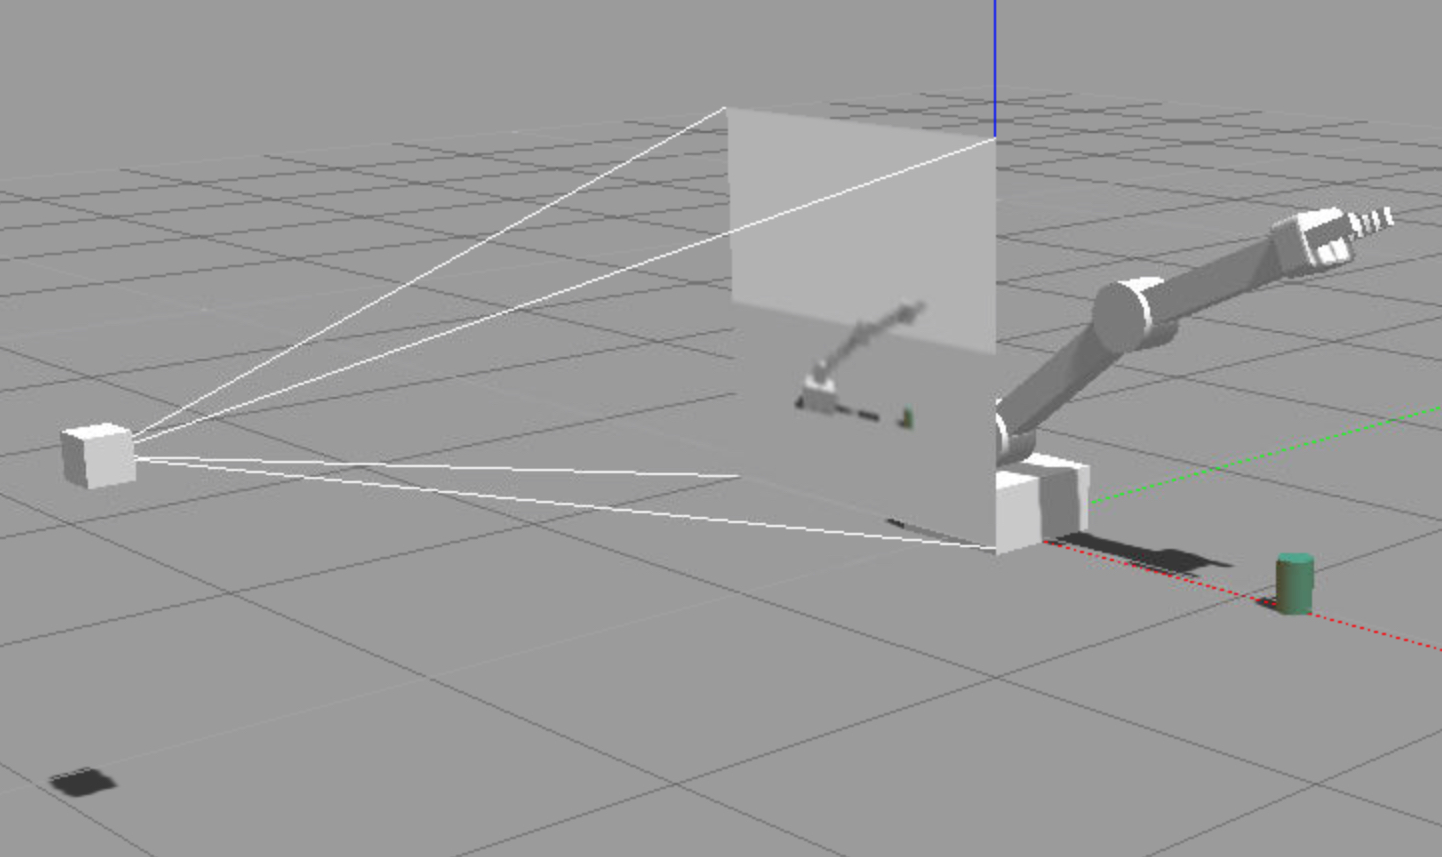
\includegraphics[width=0.6\textwidth]{environment}
\caption{Gazebo environment setup. }
\label{fig:environment}
\end{figure}

\section{Reward Function}
\subsection{Action Command}
The arm has three revolute joints which are controlled by the agent sending an action command every frame. There are two options supplied for what type of action command to send. We can either send a velocity-control action command to specify the angular velocity of a joint, or send an angle-control action command to specify the angle offset of a joint. The latter is selected in this assignment to achieve an accurate joint control.

The angle-control command has two directions, increase or decrease. Hence, the  number of actions the agent can select sums up to 6 (3 joints x 2 directions).

\subsection{Reward Value}
The agent selects one of the actions every frame. The selection is made by the action-value function of the DRQN or simply by a random choice based on an \(\epsilon\)-greedy exploration \cite{Zhan2016}. For each frame the parameters of the DRQN are updated using a reward value calculated by the reward function.

The reward function takes as input the last state of the environment and outputs the corresponding reward value. We define winning and losing scenarios in which the function returns a reward value of \(r_w=100\) and \(r_l=-10\), respectively. For the first objective, the agent wins when any part of the robot arm touches the object. For the second objective, the agent wins when only the gripper base of the robot arm touches the object, and loses if any other part touches it. In the both cases, the agent loses when any part of the arm hits the ground or the number of frames elapsed exceeds the limit value (100). If the agent wins or loses, the episode (sequence of frames) ends and a new episode starts with the environment reset to the initial state.

For each frame the function returns a interim reward based on the latest state of the agent. The function returns a positive reward if the gripper base is approaching the object, and returns a negative reward proportional to the number of frames elapsed normalized by the maximum number of episodes. This encourages the agent to move towards the object and end the episode as fast as possible. Additionally, a negative reward is returned if the amount of change in the distance between the gripper base and the object is less than 10cm. This prevents the agent from selecting an action that does not yield any progress. All the reward is multiplied by a certain coefficient. The following pseudo code shows the process of calculating the interim reward.

\begin{minted}{py}
ALPHA = 0.4
delta = lastGoalDistance - currentGoalDistance
avgDelta = avgDelta * ALPHA + (delta * (1 - ALPHA))

reward = 2.0f * avgDelta - 0.5 * currentEpisodeFrame / maxEpisodeFrame
if abs(avgDelta) < 0.01:
	reward -= 0.5
\end{minted}

\section{Hyperparameters}
List of hyperparameters and corresponding descriptions are shown in Table \ref{tab:hyperparameters}.

\begin{table}[htp]
\centering
\begin{tabular}{p{3.5cm}|p{1.5cm}|p{8.5cm}}
Hyperparameter & Value & Description \\
\hline
GAMMA & 0.9 (0.9) & Discount factor used in the Q-lerning \cite{Watkins92q-learning} update.

Lowering the value makes the agent more greedy. The default is kept to prevent from not valuing the future rewards. \\
EPS\_START & 0.9 (0.9) & Initial value of \(\epsilon\) in \(\epsilon\)-greedy exploration.

Unchanged to encourage the agent to explore in a wide range during the early frames. \\
EPS\_END & 0.001 (0.05) & Final value of \(\epsilon\) in \(\epsilon\)-greedy exploration.

Lowered significantly. Since the environment is deterministic, random explorations are no longer needed once the agent discovers a path. \\
EPS\_DECAY & (200) & Number of frames over which  \(\epsilon\) decays. \\
 & 100 & The EPS\_DECAY value for the first objective. The agent explores enough within 100 episodes for the first objective. \\
 & 150 & The EPS\_DECAY value for the second objective.  The agent explores enough within 150 episodes for the second objective. \\
INPUT\_WIDTH & 64 (512) & Image width of the camera. \\
INPUT\_HEIGHT & 64 (512) & Image height of the camera. \\
LSTM\_SIZE & 256 (32) & Number of frames fed to LSTM \cite{Hochreiter:1997:LSM:1246443.1246450} in the DRQN model. \\
OPTIMIZER & "Adam" ("None") & The name of the optimizer used for training.

Adam \cite{DBLP:journals/corr/KingmaB14} is used to allow higher learning rates. \\
LEARNING\_RATE & 0.1 (0.0) & Learning rate used by the optimizer.

A large value is set to speedup the learning process. \\
REPLAY\_MEMORY & 10000 (10000) & Number of recent frames stored for experience replay \cite{Zhan2016}.

The default value is enough to ensure randomness in the sample distribution. \\
\end{tabular}
\caption{List of hyperparameters}
\label{tab:hyperparameters}
\end{table}

\section{Results}
The reward function and hyperparameters are configured either for the first objective or for the second objective before conducting each experiment. With the configuration for the first objective, the accuracy of the arm touching the object recorded 96\% for 125 episodes, which meets the requirement. With the configuration for the second objective, the accuracy of only the gripper base touching the object recorded 81\% for 390 episodes, which also meets the requirement. The screen-shot of the results are shown in Figure \ref{fig:result}.

Due to the large learning rate, the agent finds an optimal route quite quickly (within 20 episodes at the fastest). However, the performance after the convergence highly depends on the experiences in the early frames. Because the Adam optimizer decays its effective learning rate over time, experiences in the later frames does not change the network parameter as much as those in the earlier frames. This causes the overall accuracy very low (< 60\%) when the agent fails to find an optimal solution in the earlier stage). Changing the optimizer and learning rate and/or tuning the parameters for \(\epsilon\)-greedy exploration might solve this problem.

\begin{figure}[htp]
  \centering
  \subfloat[The result for the first objective.]{
  	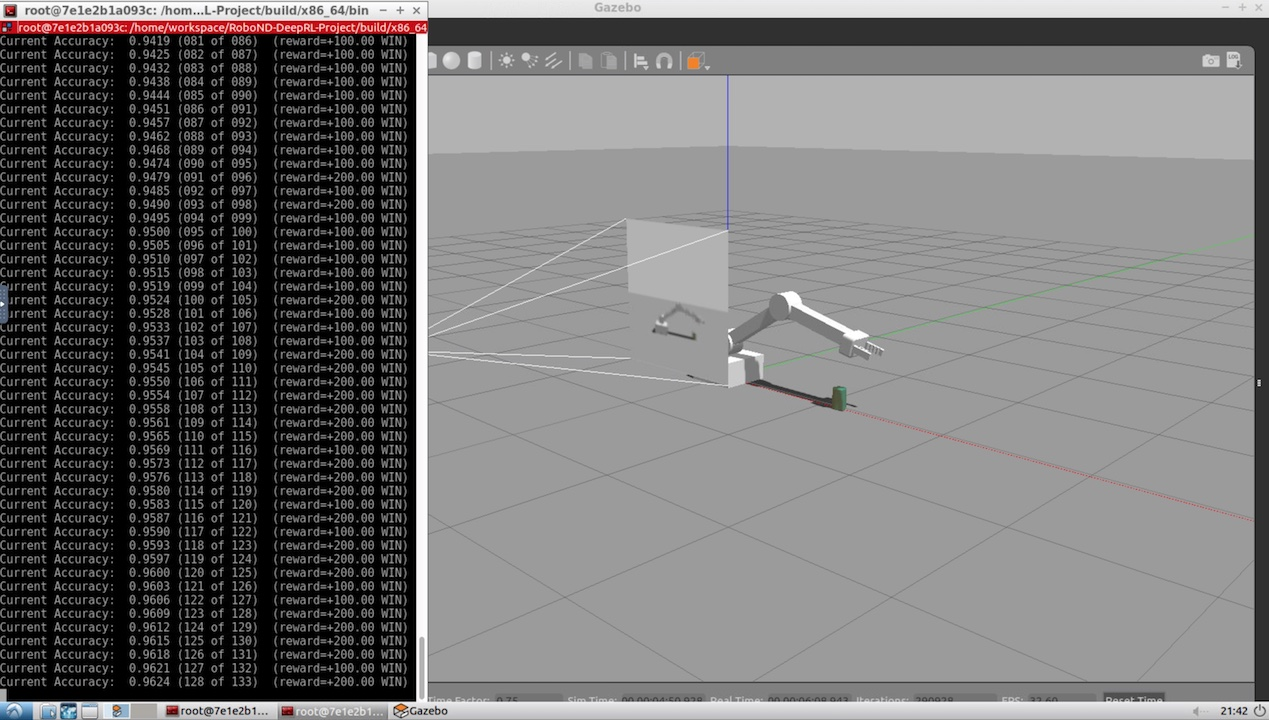
\includegraphics[width=\linewidth]{result-objective1}
    \label{fig:result-objective1}}
  \vfill
  \subfloat[The result for the second objective.]{
  	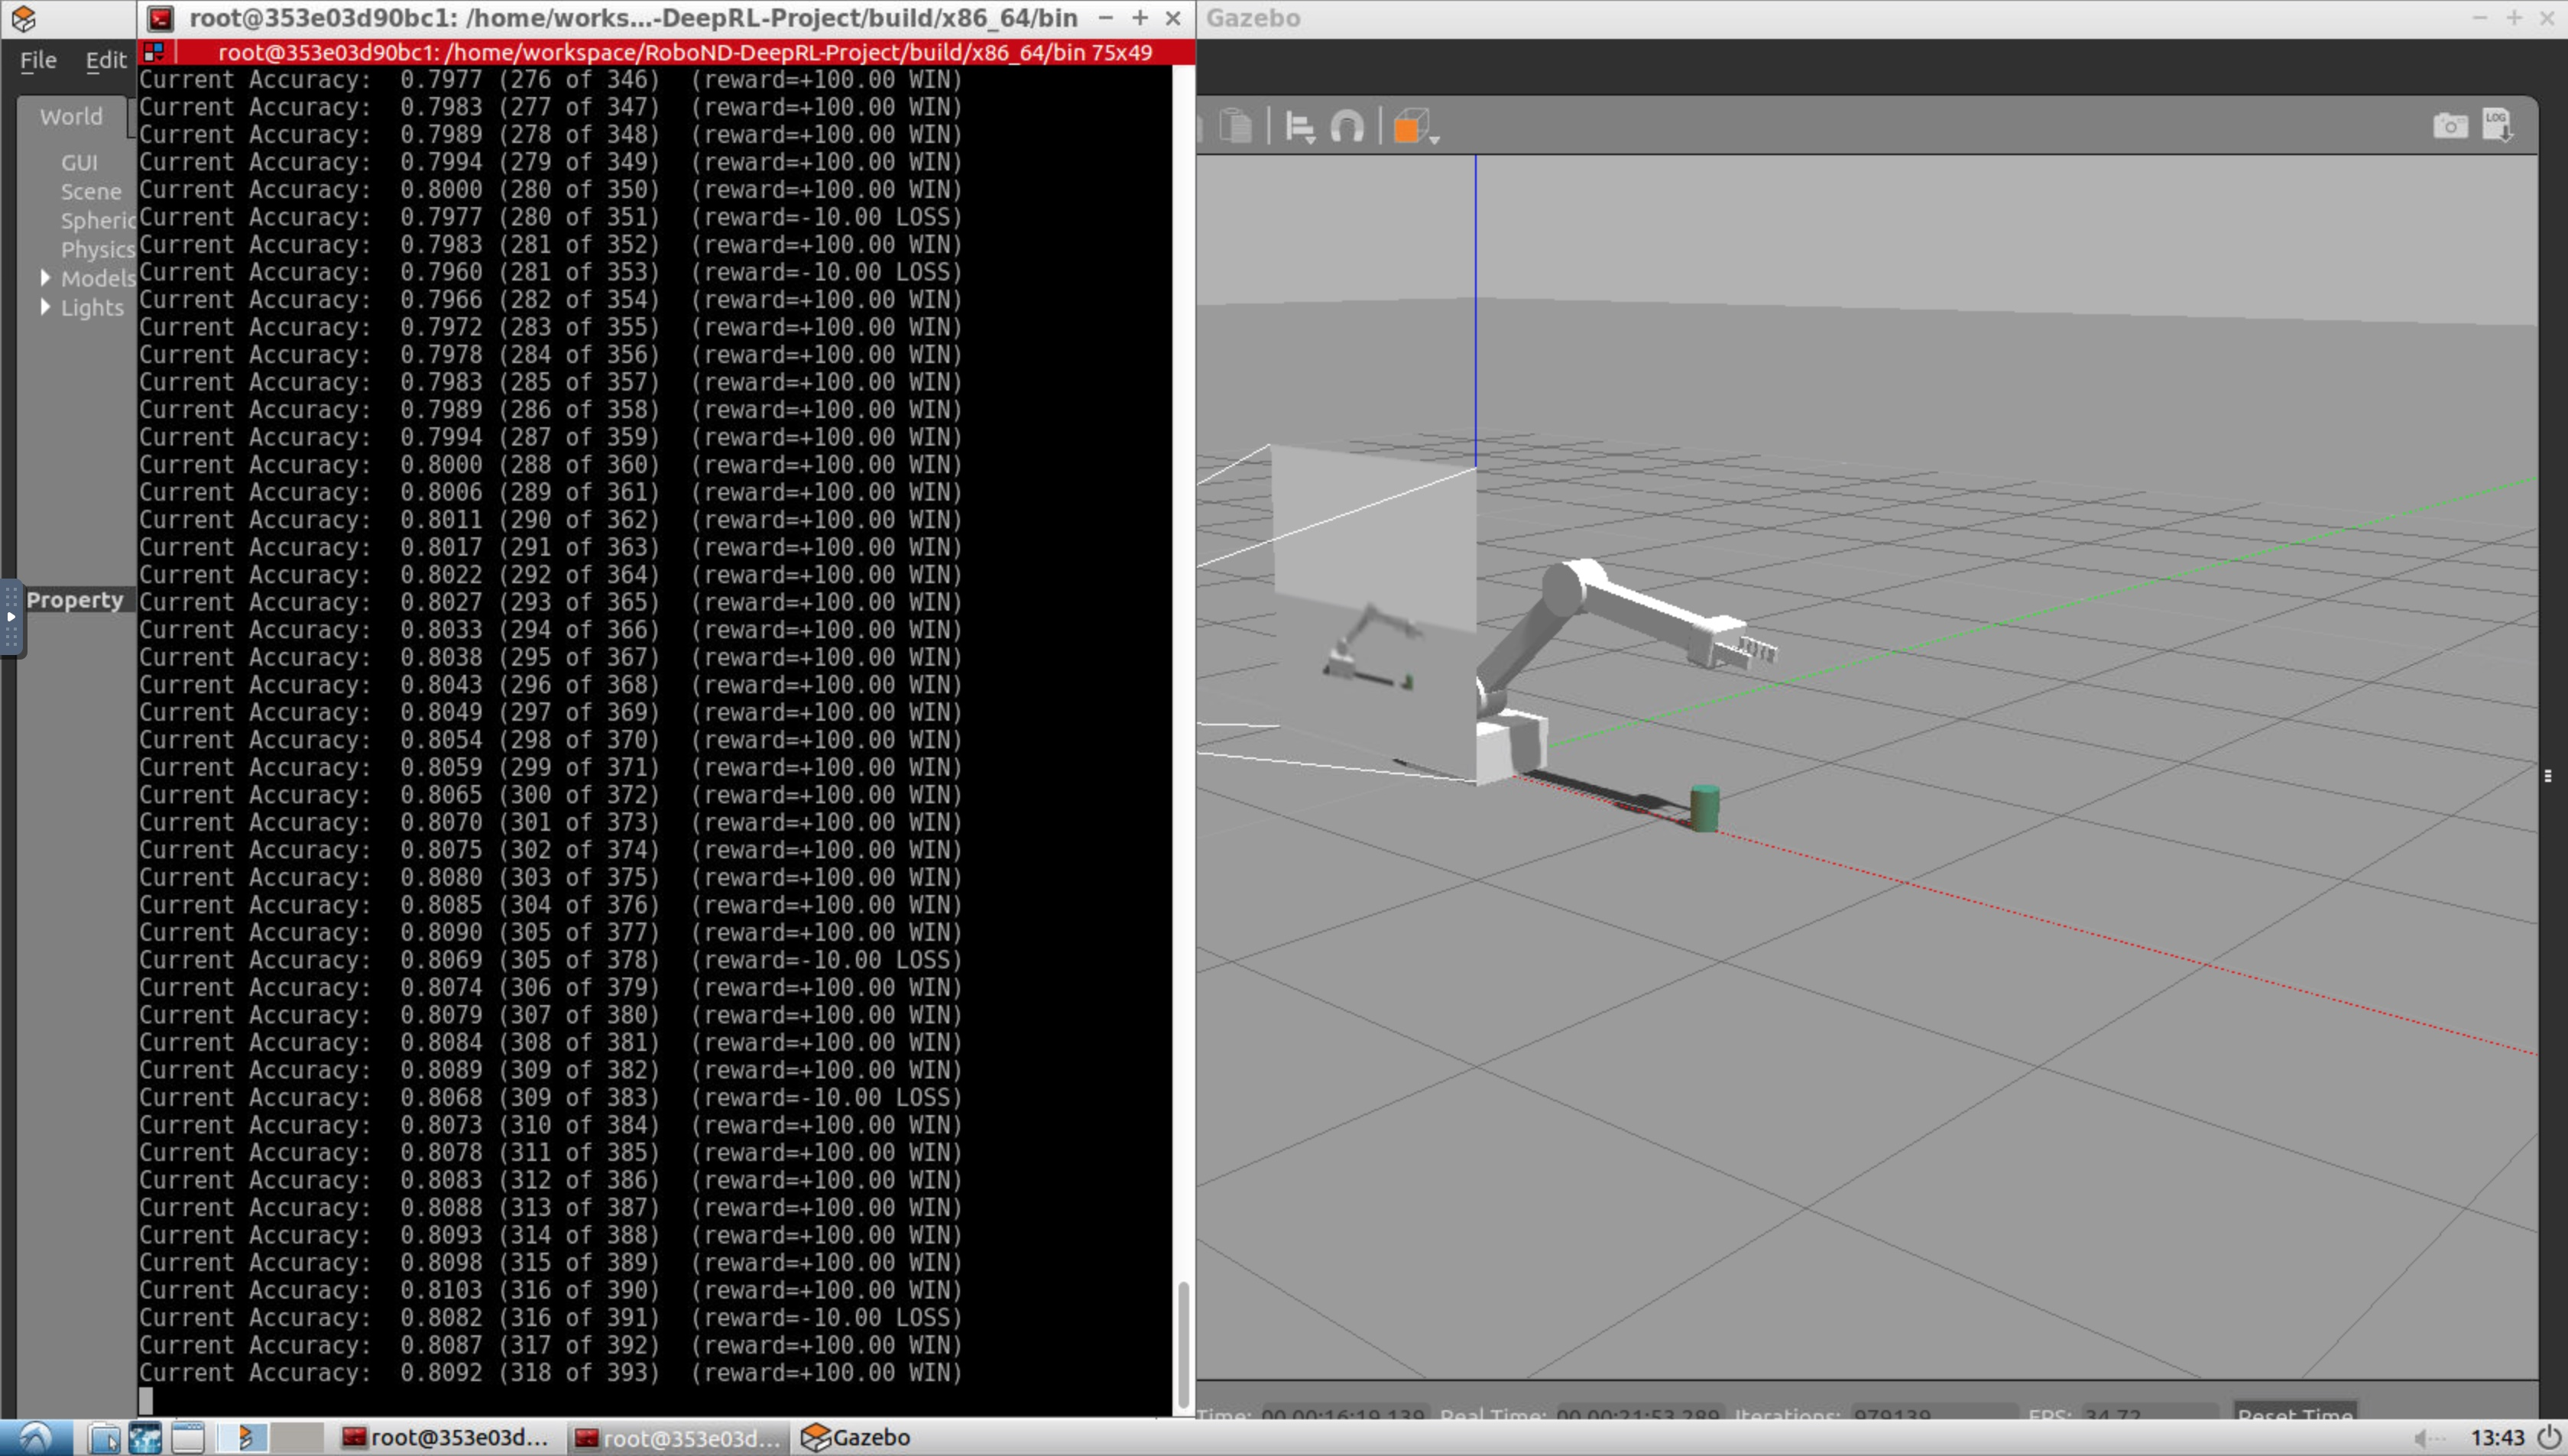
\includegraphics[width=\textwidth]{result-objective2}
    \label{fig:result-objective2}}
  \caption{A screen shot of the result for each objective.}
  \label{fig:result}
\end{figure}

\clearpage
\section{Future Work}
Future works include tuning the hyperparameters to address the problem of dependence on the experiences in earlier frames, and deal with additional challenges such as randomizing the object position and increasing the arm's degree of freedom.

\bibliographystyle{ieeetr}
\bibliography{bib}

\end{document}